\documentclass[11pt, a4paper]{article}
\usepackage{pdfpages}
\usepackage{parallel}
\usepackage[T2A]{fontenc}
%\usepackage{ucs}
\usepackage[utf8]{inputenc}
\usepackage[english,russian]{babel}
\usepackage{hyperref}
\usepackage{rotating}
\usepackage[inner=2cm,top=1.8cm,outer=2cm,bottom=2.3cm,nohead]{geometry}
%\usepackage{listings}
\usepackage{graphicx}
\usepackage{wrapfig}
\usepackage{longtable}
\usepackage{indentfirst}
\usepackage{array}
\usepackage{tikzsymbols}
\usepackage{soul}
\usepackage[ruled,vlined]{algorithm2e}
\usepackage{qrcode}
\counterwithout{figure}{section} 

\usepackage{url}
\makeatletter
\g@addto@macro{\UrlBreaks}{\UrlOrds}
\makeatother

\newcolumntype{P}[1]{>{\raggedright\arraybackslash}p{#1}}
\frenchspacing
%\usepackage{fixltx2e} %text sub- and superscripts
\usepackage{icomma} % коскі ў матэматычным рэжыме
%\PreloadUnicodePage{4}

\newcommand{\longpage}{\enlargethispage{\baselineskip}}
\newcommand{\shortpage}{\enlargethispage{-\baselineskip}}

\def\switchlang#1{\expandafter\csname switchlang#1\endcsname}
\def\switchlangbe{
\let\saverefname=\refname%
\def\refname{Літаратура}%
\def\figurename{Іл.}%
}
\def\switchlangru{
\let\saverefname=\refname%
\let\savefigurename=\figurename%
\def\refname{Литература}%
\def\figurename{Рис.}%
}
\def\switchlangen{
\let\saverefname=\refname%
\def\refname{References}%
\def\figurename{Fig.}%
}

\hyphenation{admi-ni-stra-tive}
\hyphenation{ex-pe-ri-ence}
\hyphenation{fle-xi-bi-li-ty}
\hyphenation{Py-thon}
\hyphenation{ma-the-ma-ti-cal}
\hyphenation{re-ported}
\hyphenation{imp-le-menta-tions}
\hyphenation{pro-vides}
\hyphenation{en-gi-neering}
\hyphenation{com-pa-ti-bi-li-ty}
\hyphenation{im-pos-sible}
\hyphenation{desk-top}
\hyphenation{elec-tro-nic}
\hyphenation{com-pa-ny}
\hyphenation{de-ve-lop-ment}
\hyphenation{de-ve-loping}
\hyphenation{de-ve-lop}
\hyphenation{da-ta-ba-se}
\hyphenation{plat-forms}
\hyphenation{or-ga-ni-za-tion}
\hyphenation{pro-gramming}
\hyphenation{in-stru-ments}
\hyphenation{Li-nux}
\hyphenation{sour-ce}
\hyphenation{en-vi-ron-ment}
\hyphenation{Te-le-pathy}
\hyphenation{Li-nux-ov-ka}
\hyphenation{Open-BSD}
\hyphenation{Free-BSD}
\hyphenation{men-ti-on-ed}
\hyphenation{app-li-ca-tion}

\def\progref!#1!{\texttt{#1}}
\renewcommand{\arraystretch}{2} %Іначай формулы ў матрыцы зліпаюцца з лініямі
\usepackage{array}

\def\interview #1 (#2), #3, #4, #5\par{

\section[#1, #3, #4]{#1 -- #3, #4}
\def\qname{LVEE}
\def\aname{#1}
\def\q ##1\par{{\noindent \bf \qname: ##1 }\par}
\def\a{{\noindent \bf \aname: } \def\qname{L}\def\aname{#2}}
}

\def\interview* #1 (#2), #3, #4, #5\par{

\section*{#1\\{\small\rm #3, #4. #5}}
\ifx\ParallelWhichBox\undefined%
    \addcontentsline{toc}{section}{#1, #3, #4}%
\else%
\ifnum\ParallelWhichBox=0%
    \addcontentsline{toc}{section}{#1, #3, #4}%
\fi\fi%

\def\qname{LVEE}
\def\aname{#1}
\def\q ##1\par{{\noindent \bf \qname: ##1 }\par}
\def\a{{\noindent \bf \aname: } \def\qname{L}\def\aname{#2}}
}

\newcommand{\interviewfooter}[1]{
\vskip 1em
\noindent \textit{#1}
}

\AtEndDocument{\vfill\centering \qrcode{https://github.com/fiowro/mouses/blob/main/\jobname.pdf}}

\switchlang{en}
\begin{document}

\title{1982 "--- D\'epraz/Logitech DIGIMOUSE}
\date{}
\author{~}
\maketitle
\selectlanguage{english}
Originally produced by watchmaking company Dubois Depraz SA, this mouse was designed by Andr\'e Guignard and Prof. Jean-Daniel Nicoud of the Ecole polytechnique federale de Lausanne in Switzerland in 1977. Its feature was opto-mechanical encoders, which significantly improved the original design of Douglas Engelbart. However, due to the lack of software that supported mouse control, the real spread of the D\'epraz Mouse began after 1982, when Logitech acquired its production from Dubois Depraz SA and marketed it as the first Logitech mouse, called the ``P-4 Mouse''.

In addition to Logitech, the D\'epraz Mouse was produced for Jean-Daniel Nikud's own Smaky personal computers. Also, Logitech supplied the P4 as OEM hardware for computers from a number of well-known companies: DEC, Hewlett-Packard, AT\&T, Convergent Technologies. The most common was the variant with a bright red body and black buttons (figure \ref{fig:DIGIMOUSEP4Pic}); less common are beige and white variants, as well as a few special color schemes, such as P4 for IDS in blue with white buttons and Smaky Mouse in blue with red buttons.

\begin{figure}[h]
   \centering
    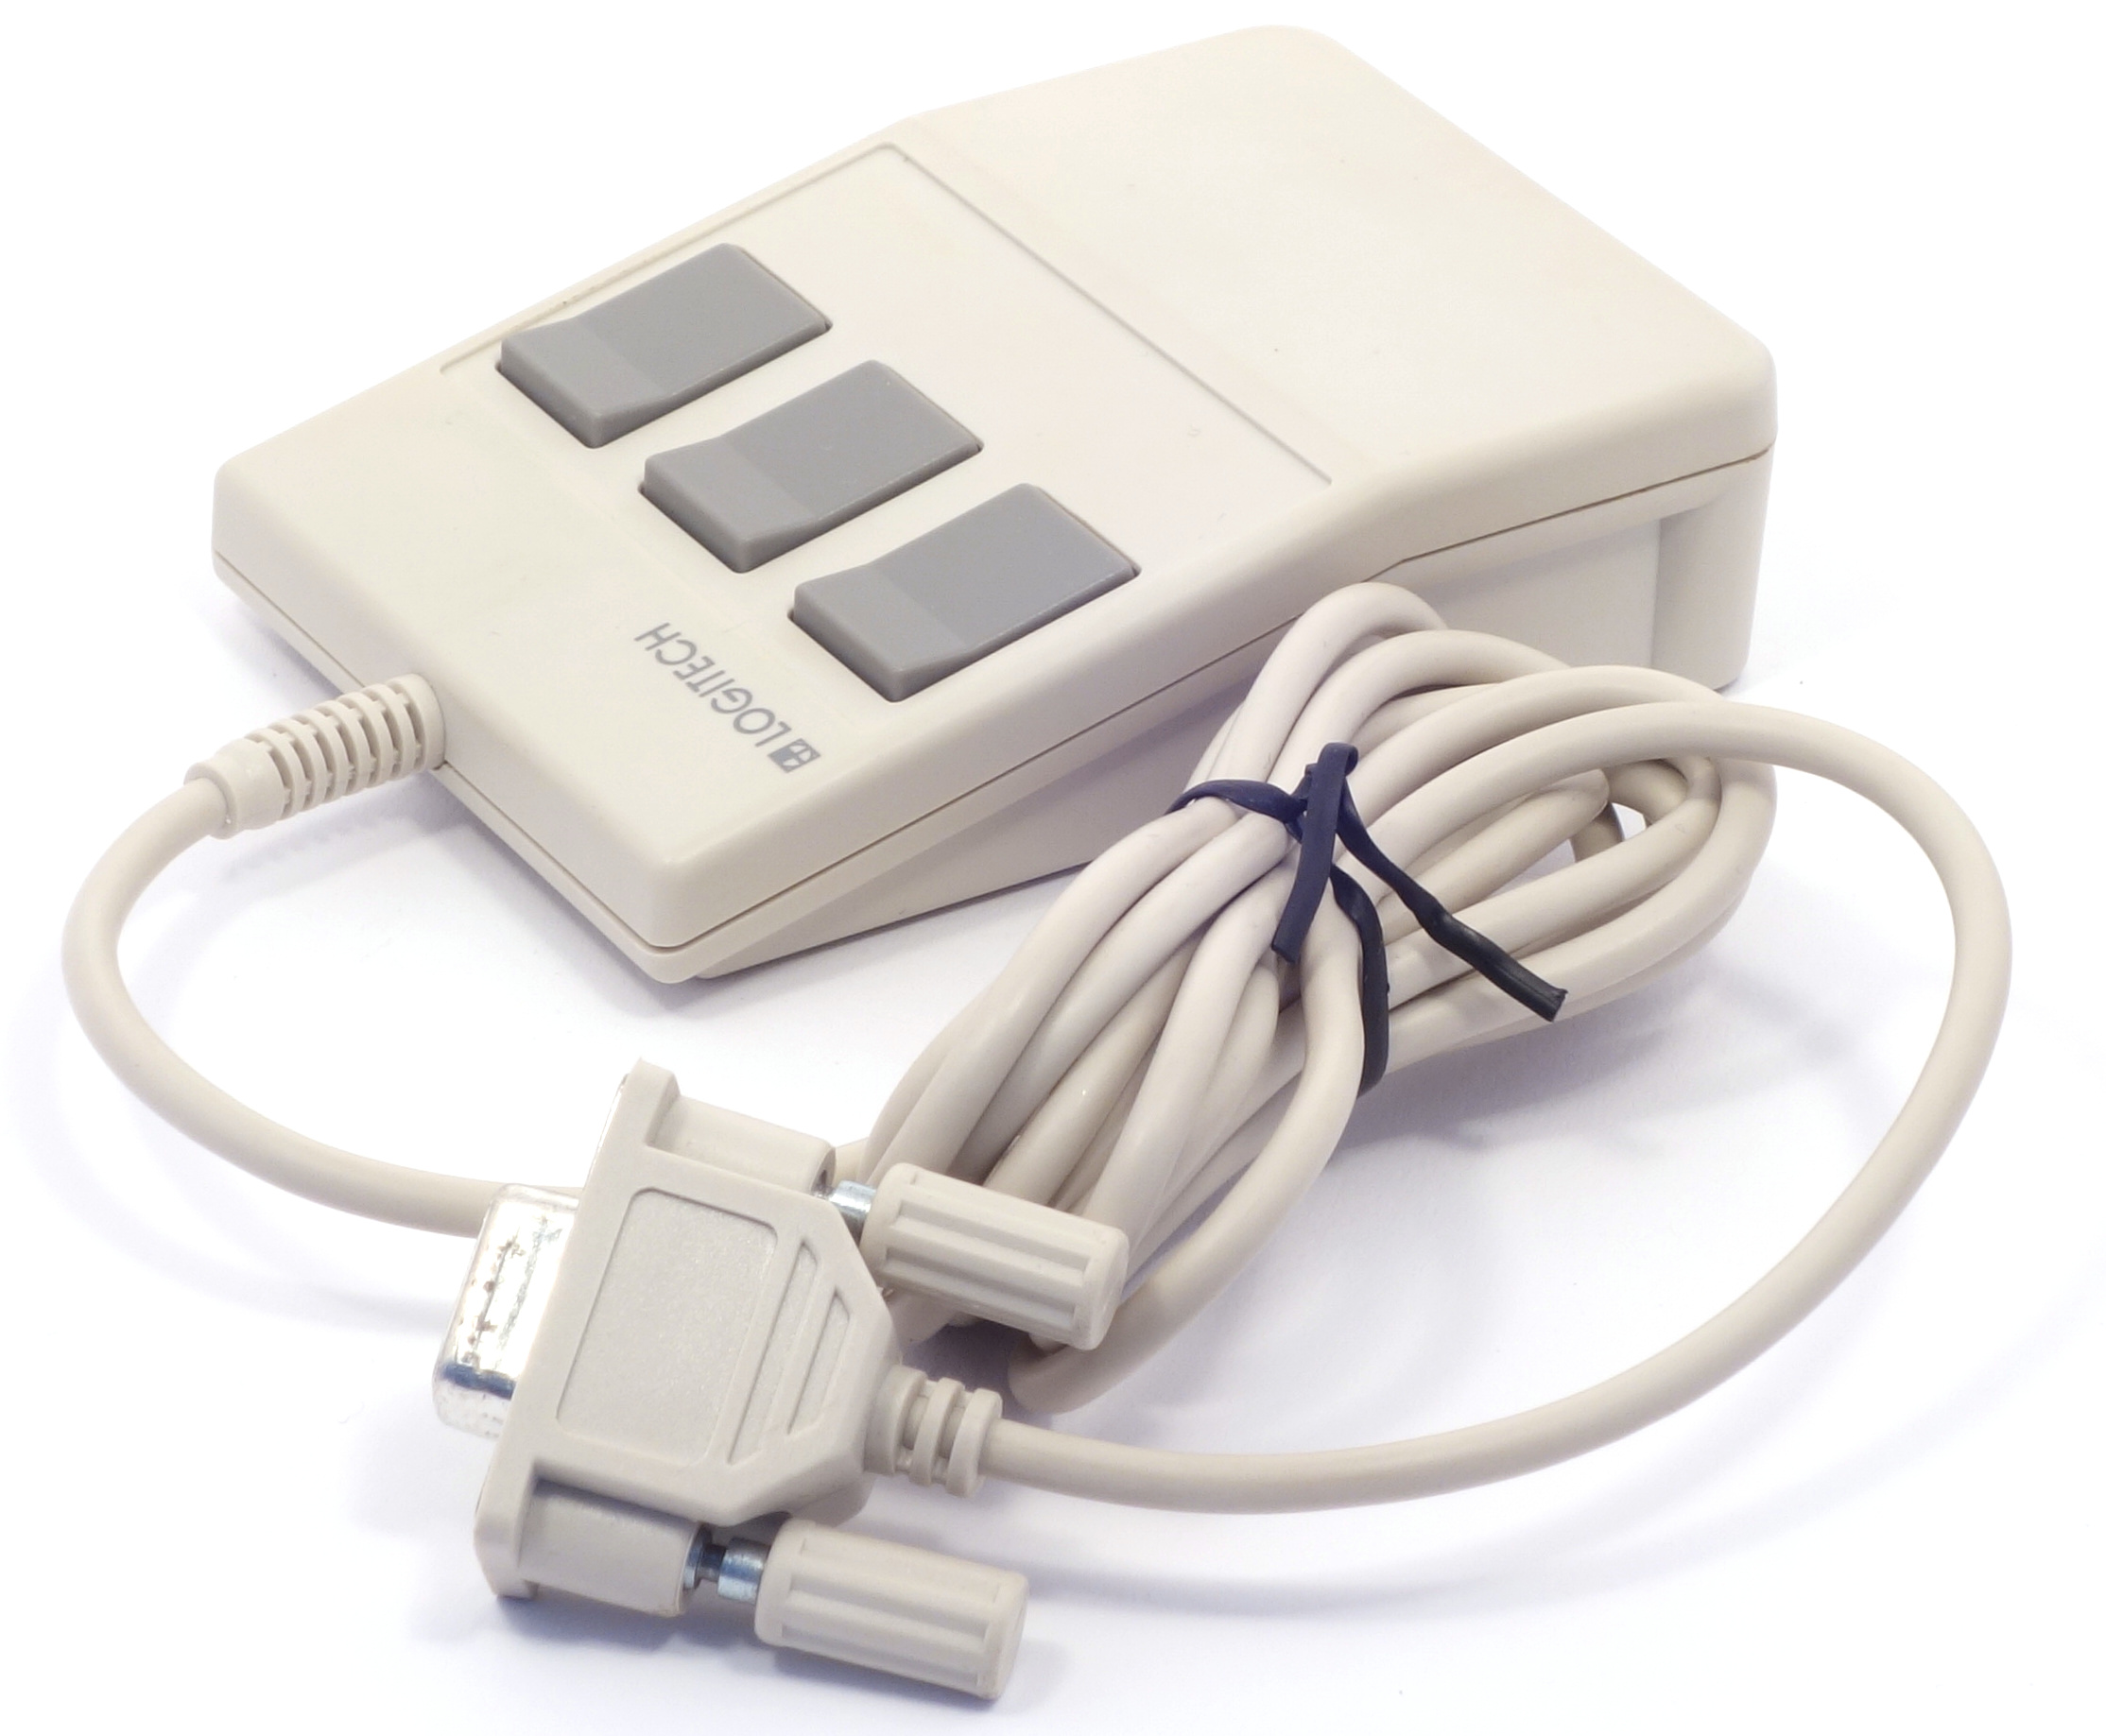
\includegraphics[scale=0.5]{1982_depraz_digimouse/pic_60.jpg}
    \caption{DIGIMOUSE}
    \label{fig:DIGIMOUSEP4Pic}
\end{figure}

The same mouse was branded in different variations as D\'epraz Mouse, Logitech P-4, DIGIMOUSE 1000 P (figure \ref{fig:DIGIMOUSEP4TopAndBottom}).

\begin{figure}[h]
    \centering
    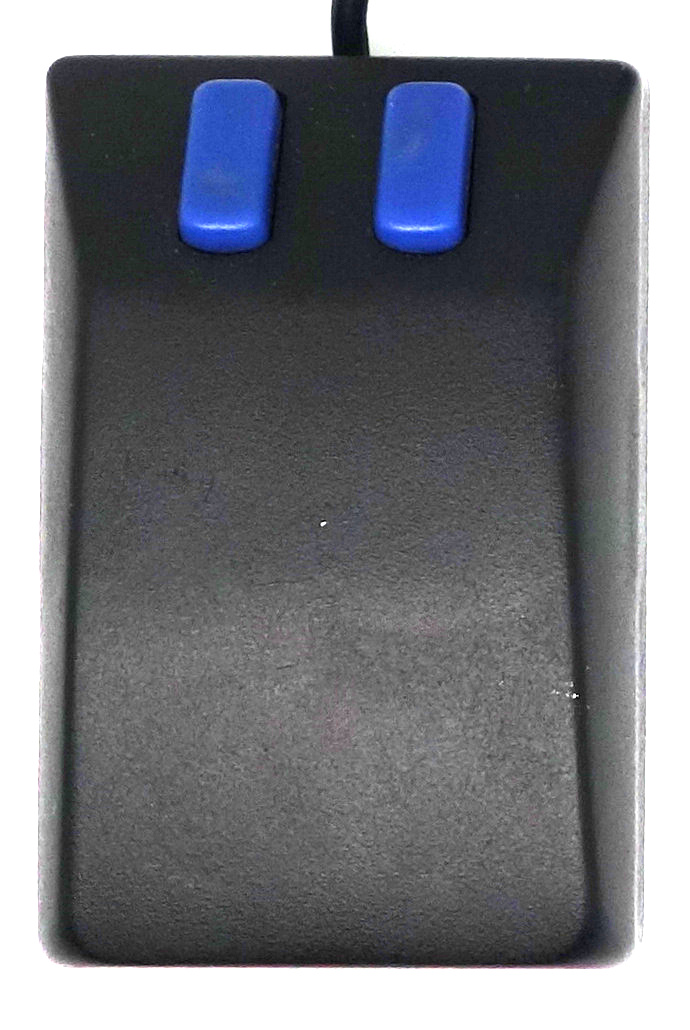
\includegraphics[scale=0.4]{1982_depraz_digimouse/top_60.jpg}
    \includegraphics[scale=0.37]{1982_depraz_digimouse/bottom_60.jpg}
    \caption{DIGIMOUSE, top and bottom views}
    \label{fig:DIGIMOUSEP4TopAndBottom}
\end{figure}

The mouse has a typical size for mice of the 1980s (figure \ref{fig:DIGIMOUSEP4Size}).

\begin{figure}[h]
    \centering
    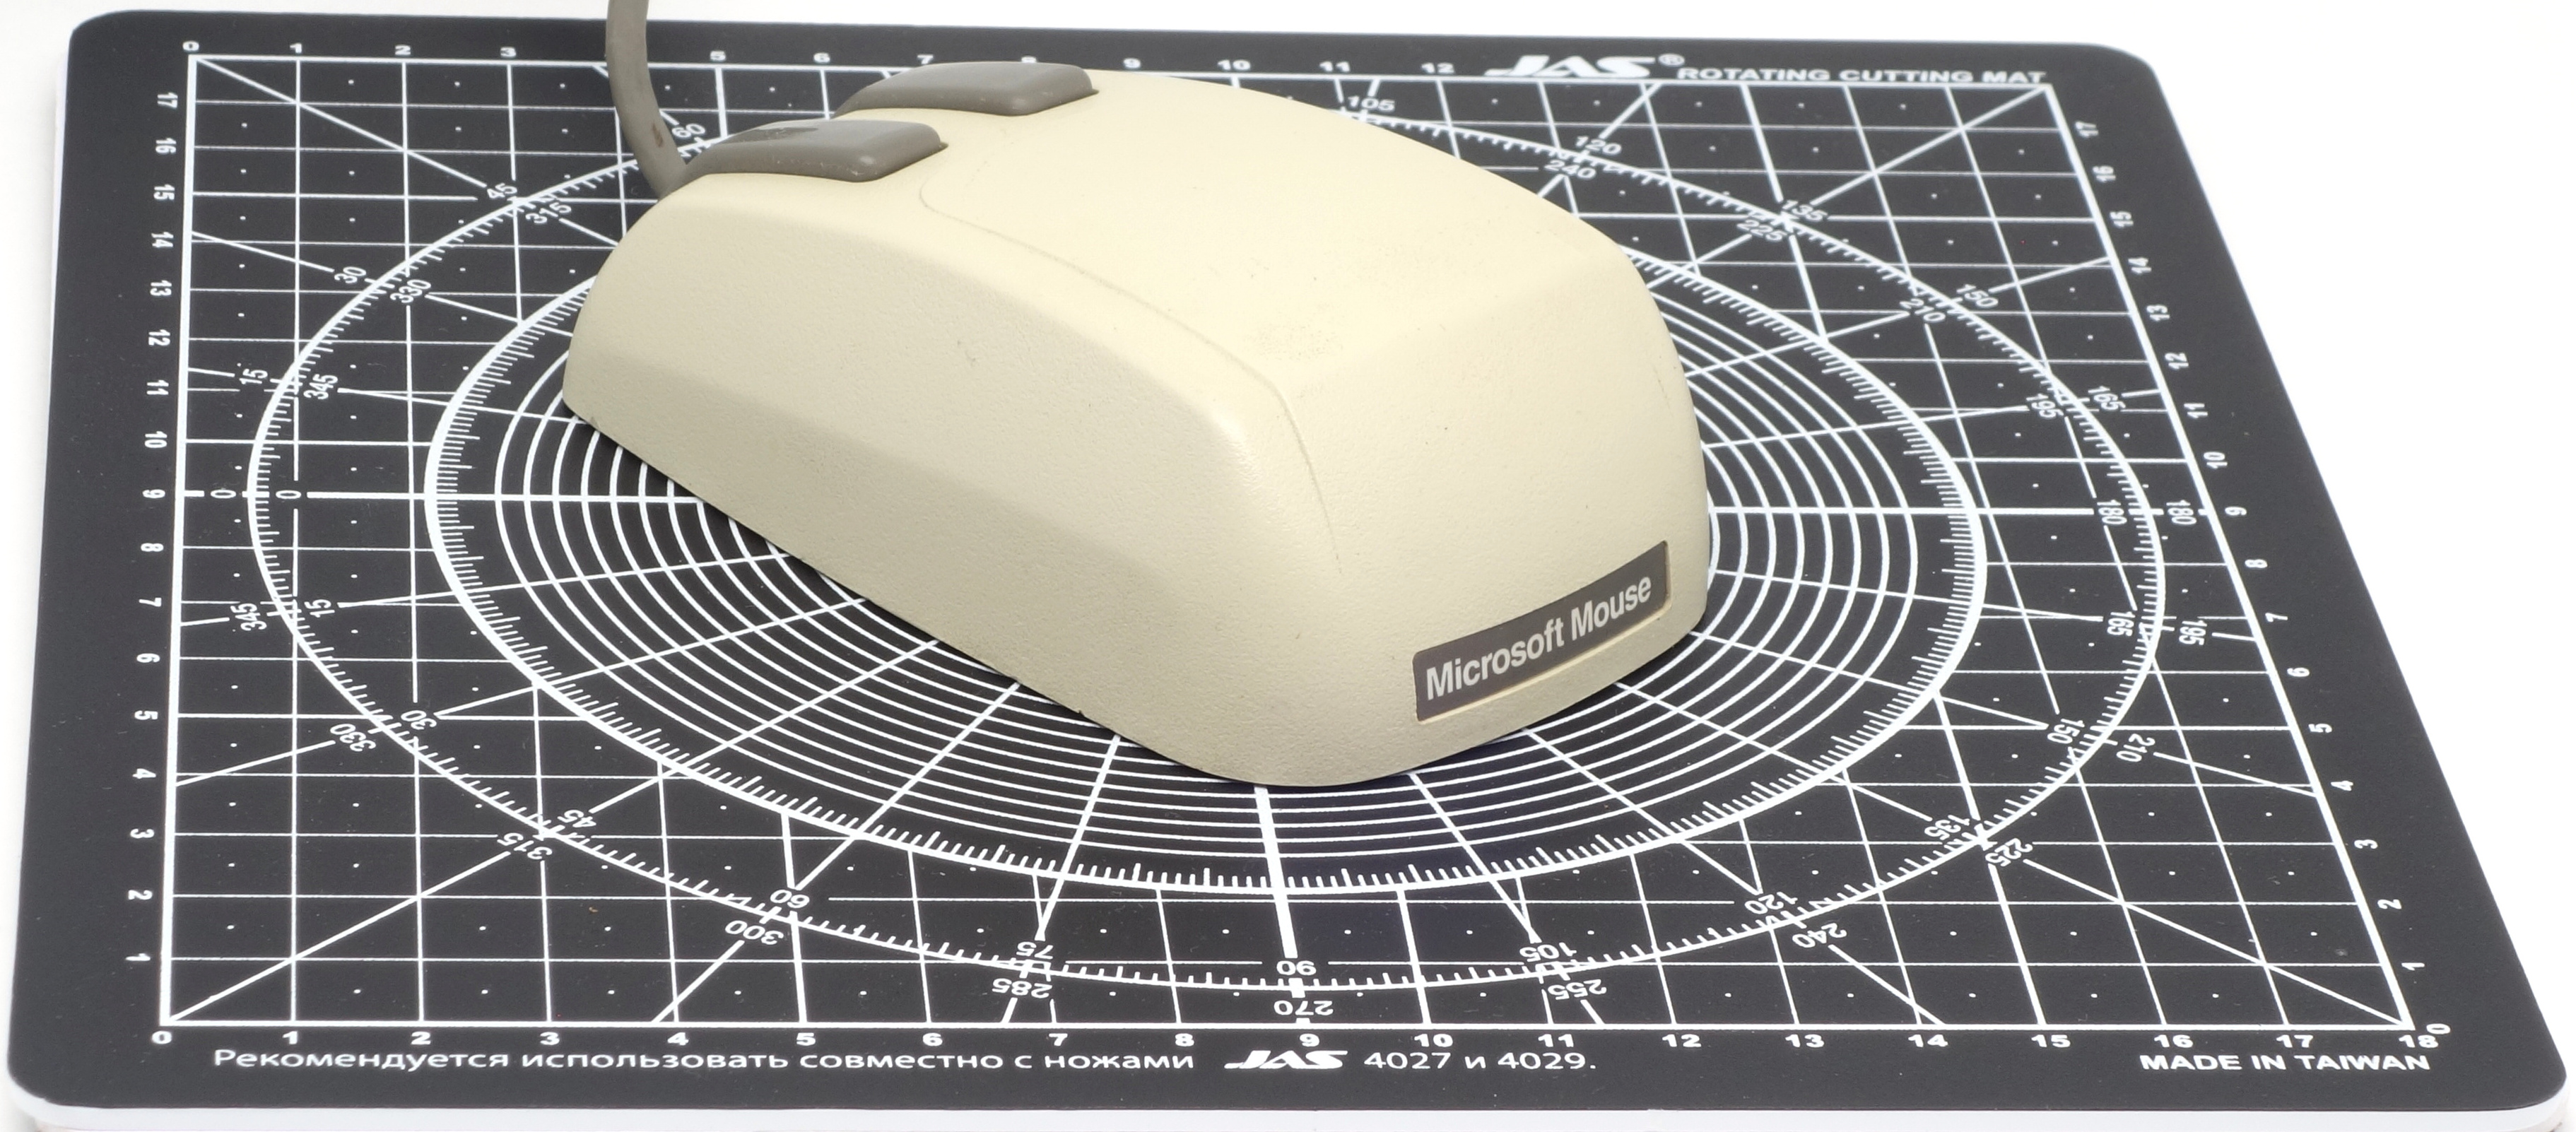
\includegraphics[scale=0.5]{1982_depraz_digimouse/size_30.jpg}
    \caption{DIGIMOUSE on a graduated pad with a grid step of 1~cm}
    \label{fig:DIGIMOUSEP4Size}
\end{figure}

The body is a 3 ½-inch hemisphere cut on the sides for easy thumb and pinky finger grip. Three spring-loaded buttons with a distinct click and tactile response to actuation are located vertically on the side of the case farthest from the user \cite{oldmouse}. Due to the fact that the buttons take up the entire front side of the case, the cable enters diagonally into the mouse. This shape was called ``dome'' and turned out to be one of the first truly successful mouse body shapes: geometric simplicity is combined with good ergonomics, making the mouse pleasant to hold in hand (figure \ref{fig:DIGIMOUSEP4Hand}). Owners of small hands can easily rest their wrist on the table or lift it up when necessary to use the buttons.

\begin{figure}[h]
    \centering
    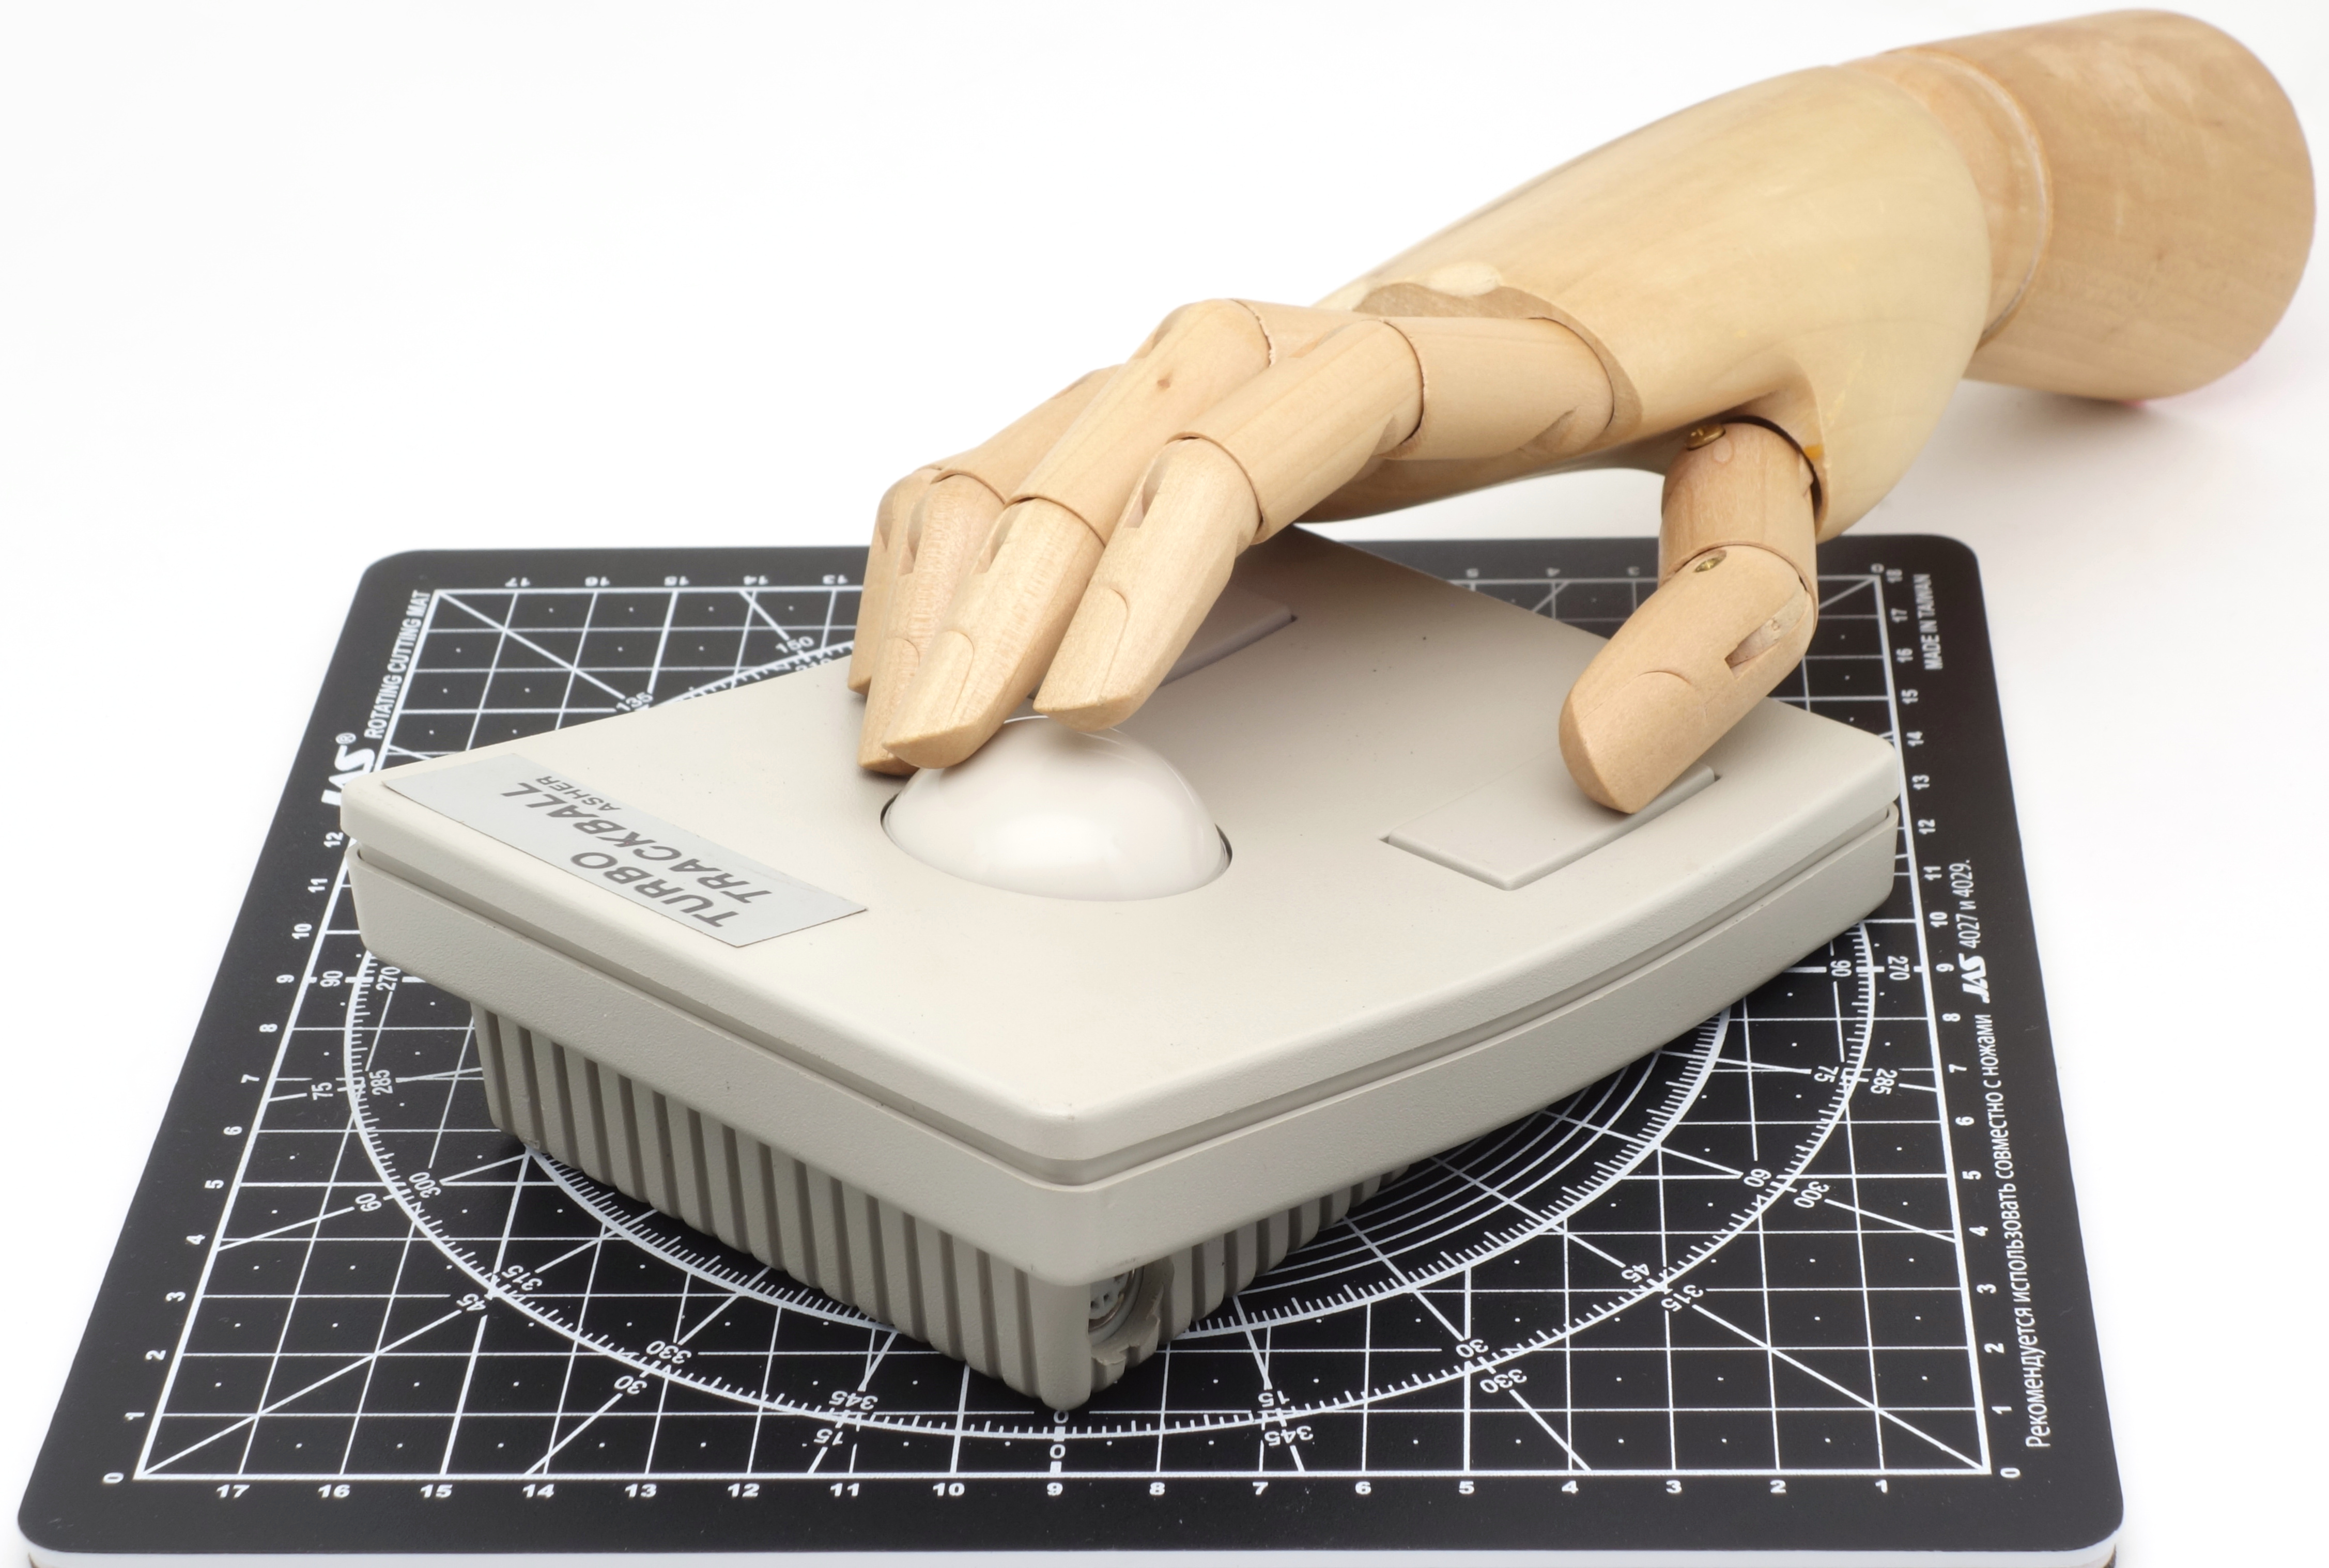
\includegraphics[scale=0.5]{1982_depraz_digimouse/hand_30.jpg}
    \caption{DIGIMOUSE with a human hand model}
    \label{fig:DIGIMOUSEP4Hand}
\end{figure}

The mouse has a 381 DPI resolution. Since 1984, as an additional accessory, these mice were sometimes equipped with a special LogiMate \cite{oldmouse} converter, which allowed the mouse to be connected not to a separate adapter with a bus interface, but to a keyboard cable. With this connected, moving the mouse resulted in generating cursor key codes:  the resolution was 12 keypresses per inch horizontally and 6 keypresses vertically by default, which was designed to work in 80x25 character text mode. PC Magazine's review noted that using a mouse in standard mode made it possible to move the cursor in a text editor seven times faster than using the corresponding keys on the keyboard (however, it took getting used to the fact that as a result of a slight movement of the mouse over the rightmost position, the text editor cursor immediately jumped to the left position of the next line). For obvious reasons, this use of the mouse did not require a driver; however, its use gave the possibility of additional settings "--- for example, it allowed to set the resolution of the LogiMate adapter in the range of 1--100 keypresses per inch, as well as reassign the action of the mouse keys (key codes F8, F9 and F10 were generated by default) \cite{DIGIMOUSE}.

 \begin{figure}[h]
    \centering
    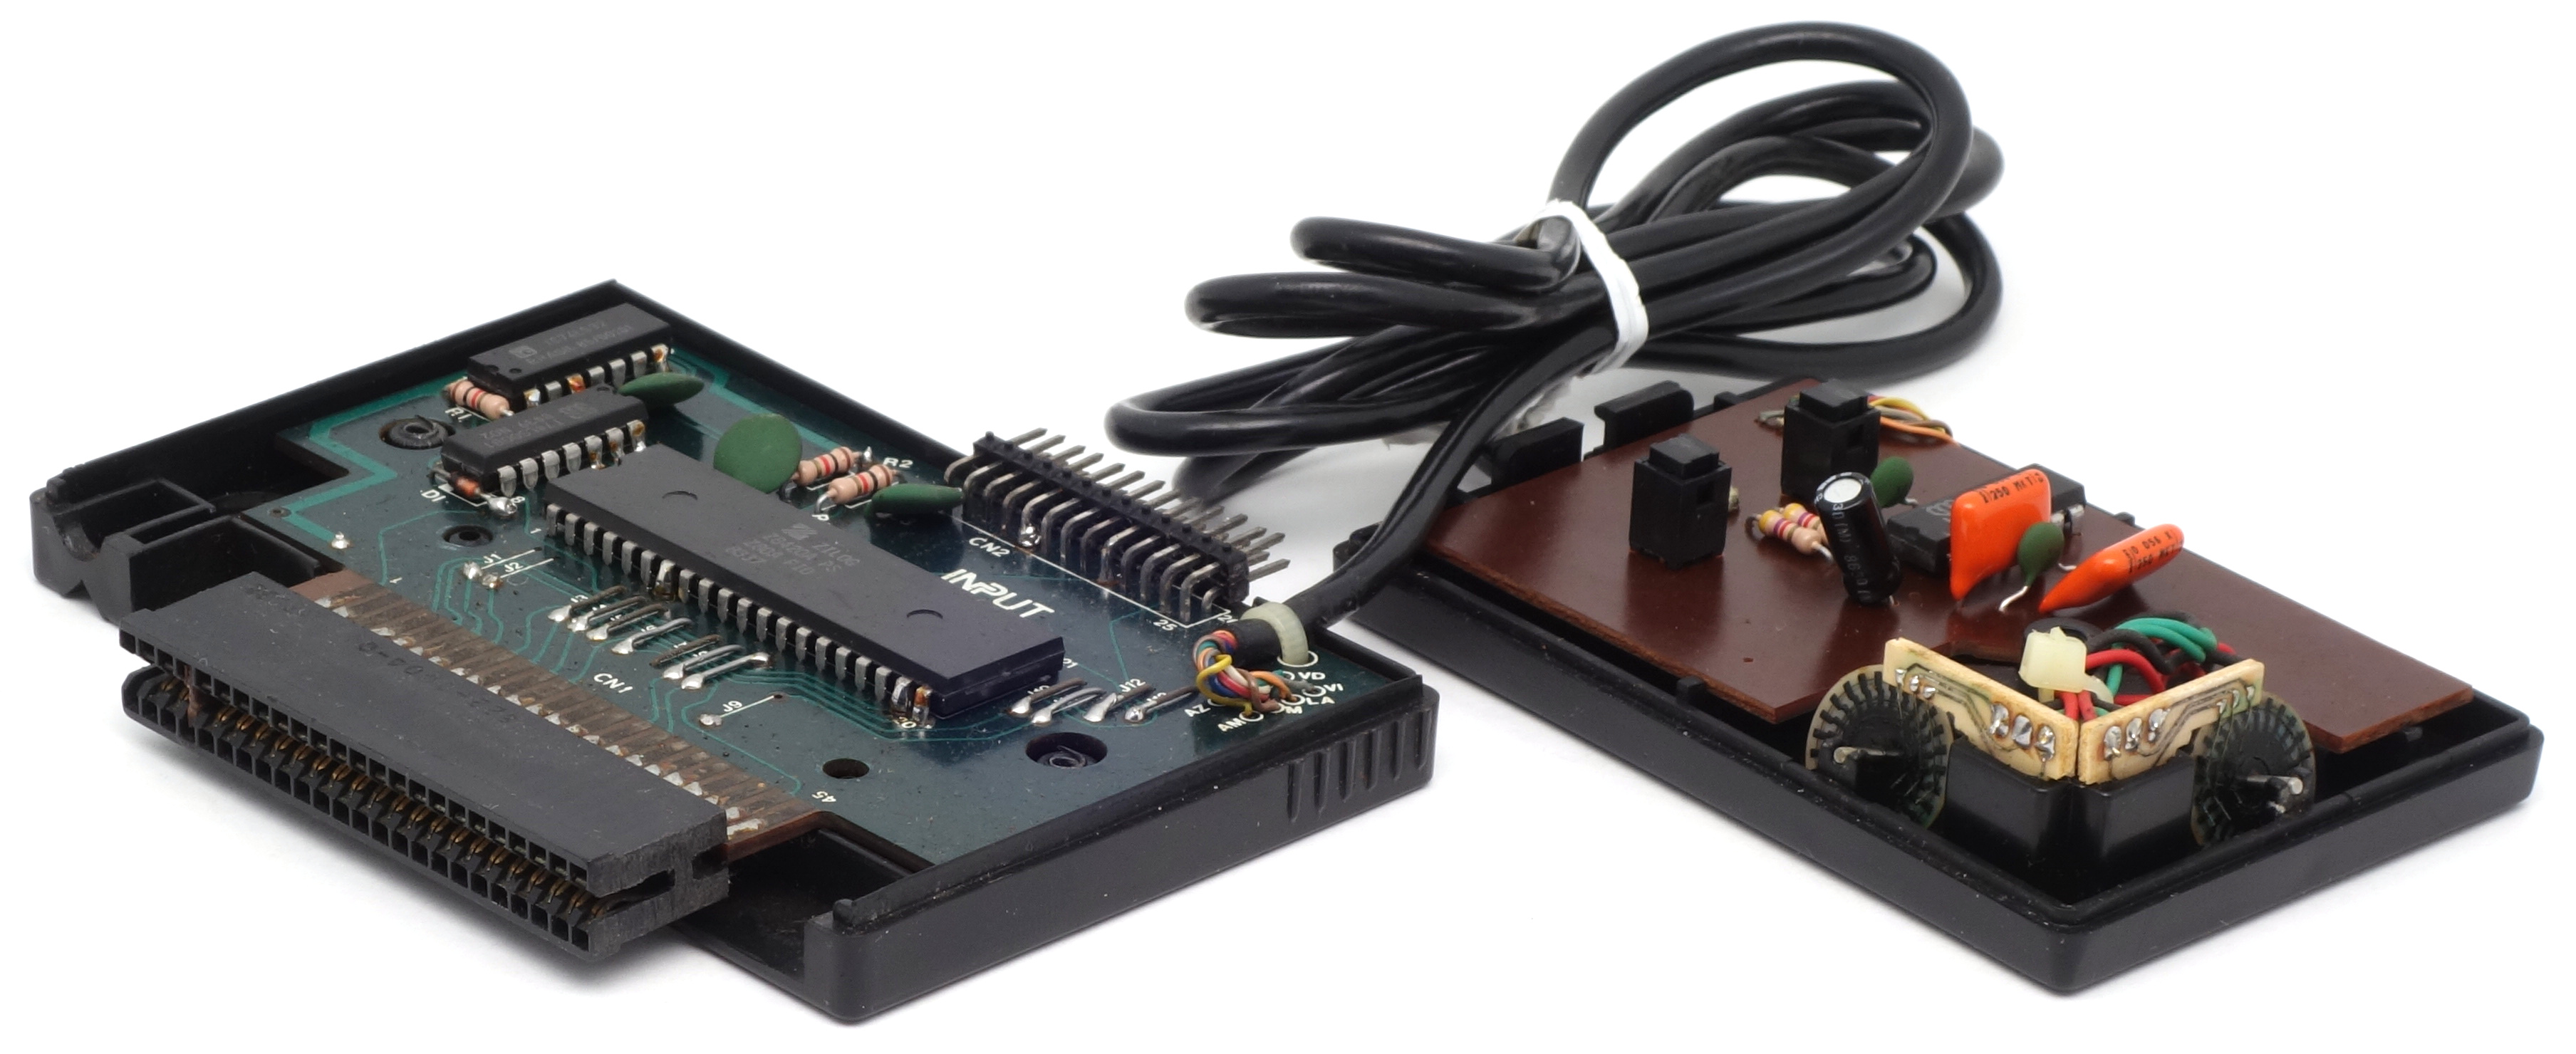
\includegraphics[scale=0.75]{1982_depraz_digimouse/inside_60.jpg}
    \caption{DIGIMOUSE disassembled}
    \label{fig:DIGIMOUSEP4Inside}
\end{figure}

The internal structure of the mouse is shown in figure \ref{fig:DIGIMOUSEP4Inside}. As already mentioned, this mouse uses optomechanical encoders. Optocouples are similar to those in mice from the 90s; however, the optical interrupter disk is made of metal and additionally equipped with a fixed mask that reduces the area of flare. During Logitech's production, the original design of the D\'epraz Mouse underwent some changes: in particular, the material of the roller cover and the original metal ball \cite{oldmouse} were replaced with plastic.

The most active sales of this mouse are from 1982 to 1984 (production ceased in the mid-80s with the release of the very popular inexpensive Logitech C7 model), and the original retail price was \$295. In a number of ways, the D\'epraz Mouse was a significantly more technologically advanced device than other mice of the first half of the 1980s. The combination of technological superiority, rather high price, and good ergonomics made this manipulator legendary. As a result of such popularity, in the first half of the 1990s, the "dome mouse" story continued unexpectedly with the release of two P4 clones: an almost complete visual copy from Sunnyline called Hit Mouse\cite{sunnyline}, as well as a transparent Crystal Clear Mouse manufactured by Suncom\cite{suncom}.

As you can see (figure \ref{fig:HitMousePic}), Hit Mouse is copying the exterior of P4 as close as possible. It was developed for the Amiga computers. In fact, the most noticeable change from DIGIMOUSE is the removable latch turnable ring cover of the ball, common in the 1990-s for being really handy to remove dirt and clean rollers.

\begin{figure}[h]
   \centering
    \includegraphics[scale=0.5]{1982_depraz_digimouse/hitmouse_pic_30.jpg}
    \caption{Sunnyline Hit Mouse}
    \label{fig:HitMousePic}
\end{figure}

Of course, the copying was only related to the exterior (the most common was the red case and black buttons, although the article in Amiga Kickstart also mentions \cite{sunnyline} a transparent version in addition to Suncom's variant). Internally, Hit Mouse is close to typical optomechanical mice of the mid-90s (figure \ref{fig:HitMouseInside}). Taking into account the fact that Hit Mouse was produced in 1991-1992, technically it can be considered a very relevant device for its time.

However, the domed shape, which proved to be an extremely successful solution among mice of the 80s, no longer aroused such enthusiasm among users of the 90s. The Amiga Kickstart short review described this design as very unusual, taking time to get used to \cite{sunnyline}.

 \begin{figure}[h]
    \centering
    \includegraphics[scale=0.7]{1982_depraz_digimouse/hitmouse_inside_30.jpg}
    \caption{Sunnyline Hit Mouse disassembled}
    \label{fig:HitMouseInside}
\end{figure}

\begin{thebibliography}{9}
\bibitem {DIGIMOUSE} J. Taylor. Faster then a speeding cursor key. // PC Magazine, V. 3, No. 2, February 7, 1984. -- p. 243-245 \url{https://archive.org/details/PC-Mag-1984-02-07/page/n243/mode/2up}
\bibitem {oldmouse} D\'epraz / Digimouse mouse $\sim$ oldmouse.com \url{https://web.archive.org/web/20211019061819/https://www.oldmouse.com/mouse/logitech/digimouse.shtml}
\bibitem {sunnyline} A. Kramer. PIEP-SHOW. M\"ause im Vergleich. Hit-Mouse II // Amiga Kickstart No. 10, Oktober, 1991. -- p. 52-54 \url{https://archive.org/details/amiga-kickstart-91-10/page/52/mode/2up}
\bibitem {suncom} Crystal mouse, Suncom Technologies, 1991, USA. Mice Farm on Instagram. \url{https://www.instagram.com/p/CXYkzSpoqnL/}
\end{thebibliography}
\end{document}
